% Working manuscript, revised 2026-09-15. Pending cells are NOT measured results.
% Read 06_MANUSCRIPT_REVISION_AND_FIGURES_ZH.md before final submission.
% Compile from this directory. Official ieeeconf class; 8 pages INCLUDING refs.
\documentclass[letterpaper,10pt,conference]{ieeeconf}
\IEEEoverridecommandlockouts
\overrideIEEEmargins
\usepackage{graphicx,booktabs,amsmath,amssymb,tabularx}
\usepackage{tikz}
\usetikzlibrary{arrows.meta,positioning,fit,backgrounds}
\usepackage{cite}
\usepackage{url}
\usepackage{xcolor}
\newcommand{\pending}{\textit{pending}}
\newcommand{\figplaceholder}[2]{\fbox{\parbox[c][#1][c]{0.94\linewidth}{\centering\small #2}}}
\title{Beyond the Takeover: Human-Corrected Predictive Learning for World--Action Models}
% Named author version requested by the authors.
\author{Fenghao Liu$^{1,*}$, Yunpeng Zhu$^{2,*}$, Lixi Fan$^{3,*}$,\\
Zhangyuan Wang$^{2,\dagger}$\thanks{$^{*}$Equal contribution. $^{\dagger}$Corresponding author. $^1$University of Michigan; $^2$Westlake University; $^3$Zhejiang University.}}
\begin{document}
\maketitle
\thispagestyle{empty}
\pagestyle{empty}

\begin{abstract}
World--action models (WAMs), such as AHA-WAM, advance general-purpose manipulation by jointly modeling visual scene dynamics and actions. However, demonstration-trained WAMs remain limited by the coverage and quality of their training data, leaving closed-loop interaction experience untapped. Interactive learning frameworks such as HG-DAgger can supply corrective behaviors through human takeovers at critical moments of autonomous execution. Yet for WAMs that predict actions and video in temporal context, these short interventions can omit the visual evidence needed to interpret the evolving physical scene. We present an interactive learning framework for memory-based WAMs that transforms human-gated real-robot deployments into temporally contextualized corrective experience. Its core mechanism, human-corrected predictive policy self-improvement, couples human-supervised action learning with prediction of observed visual continuations. Pre-takeover observations preserve memory context, human corrections specify the behavior to imitate, and eligible post-handback video extends visual supervision without treating autonomous actions as expert labels. Preliminary real-robot results show improved completion on cylinder and power-adapter insertion, with qualitative evidence of recovery from multiple execution errors. We further introduce a recovery-oriented prediction--behavior analysis to investigate whether task-relevant video prediction fidelity is associated with real-robot recovery performance.
\end{abstract}

\section{Introduction}
World--action models (WAMs) couple visual forecasting with action generation, bringing predictive representations into manipulation~\cite{videovla,ahawam}. AHA-WAM uses a low-frequency video planner and a higher-frequency action executor with reusable visual context~\cite{ahawam}. Yet demonstration-trained policies can still fail after small deviations in precision insertion.

The promise of predictive robot policies is not simply to reproduce an observed action, but to connect what the robot sees, how the scene evolves, and what it should do next. Precision manipulation exposes the distance between this promise and deployment: an approach that looks nearly correct can end in a failed insertion, after which completing the task requires a different behavior from the nominal demonstration. Richer visual representations alone do not ensure that such behavior is present in the training distribution. Three limitations motivate interactive post-training.

\textit{Compounding distribution shift.} Small deviations in grasp or approach move the learner away from demonstrated states; subsequent actions can amplify the mismatch~\cite{dagger}. Improving nominal trajectory imitation does not directly supply supervision at these newly encountered states.

\textit{Missing corrective behavior.} Successful demonstrations may omit the search, retreat, and realignment needed after a misplaced approach. Human interventions provide locally relevant behavior at precisely these manipulation bottlenecks~\cite{iwr}.

\textit{Unused deployment experience.} A fixed demonstration dataset excludes the consequences of the learner's own execution. Human--robot interaction makes these observations available for further learning~\cite{sirius}, raising a question specific to predictive policies: which parts of a mixed-control trajectory should supervise behavior, and which should support world modeling?

We study this question through cylinder and power-adapter insertion on a low-cost robot. Both tasks require correcting geometric misalignment, while their different visual configurations provide contrasting settings for examining predictive learning and task completion.

Human-gated DAgger supplies corrective actions at learner-visited states by allowing an operator to take over and return control~\cite{hgdagger}. For a memory-based WAM, however, the expert-action interval is only part of a training example. Cropping a short intervention can remove its preceding visual context and leave too few future frames for prediction. The adaptation problem is therefore not only which actions to imitate, but which surrounding observations to retain.

Our central observation is that \emph{the boundary of an expert action label need not delimit useful visual evidence}. We preserve pre-takeover observations as context and extend eligible video targets along recorded successful continuations, while restricting expert actions to human control. Original demonstrations are replayed alongside corrections to update the existing WAM. Figure~\ref{fig:framework} presents the interaction workflow; Figure~\ref{fig:method} specifies its temporal supports.

We call this perspective \emph{Beyond the Takeover}: a short human intervention anchors learning, while its surrounding real-world context supplies evidence about how the correction is situated and how the scene subsequently evolves. This separates the scarcity of expert action labels from the availability of visual experience. The resulting framework connects interactive imitation with predictive post-training, using the existing WAM as both a policy and a model of visual continuation.

Our contributions are threefold:
\begin{itemize}
\item \emph{An interactive learning framework for WAMs.} We integrate human-gated real-robot interaction, temporally contextualized correction construction, and demonstration replay to adapt an existing WAM at the deviations encountered during precision manipulation.
\item \emph{Human-corrected predictive policy self-improvement.} We combine human action supervision, observed history, and future-video self-supervision, enabling short corrections to guide learning from longer mixed-control experience while preserving distinct supervision boundaries.
\item \emph{Understanding how video prediction supports error recovery.} We investigate the interplay between predictive fidelity and corrective behavior through temporal-support ablations and checkpoint-level comparison of held-out video prediction with real-robot success. Cylinder exhibits aligned predictive and behavioral improvement, while power adapter reveals a prediction--execution gap that delineates the limits of this relationship.
\end{itemize}

\begin{figure*}[t]
\centering
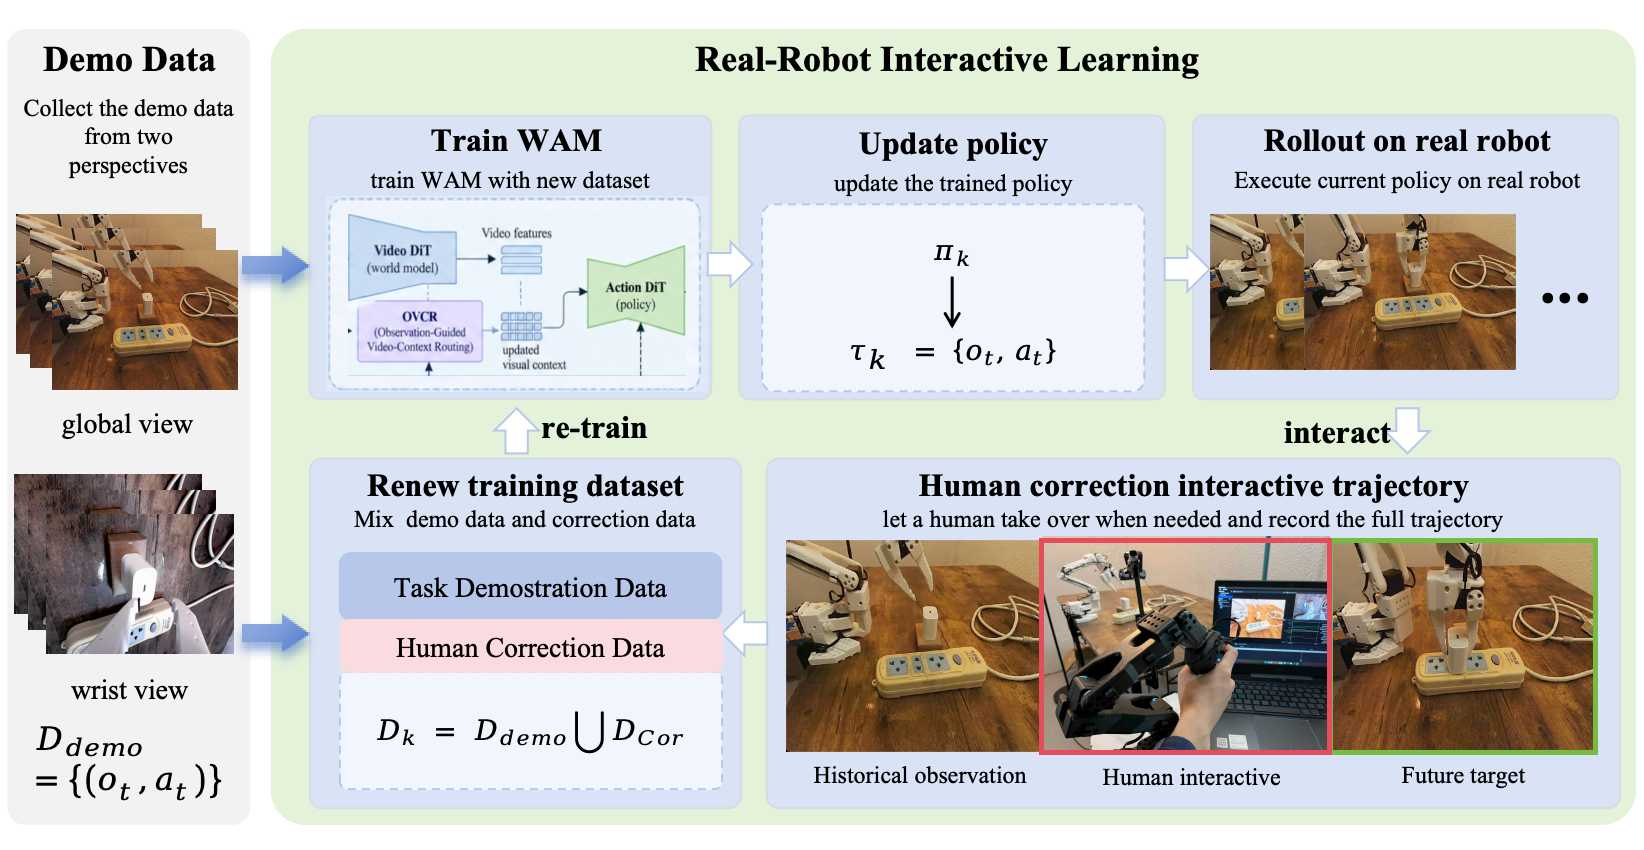
\includegraphics[width=\linewidth]{figures/interactive_learning_framework.jpg}
\caption{Real-robot interactive learning framework. Two-view demonstrations initialize the WAM. Human takeovers and surrounding observations provide corrective experience for post-training with demonstration replay. The diagram depicts an iterative workflow; the present experiments evaluate one correction round.}
\label{fig:framework}
\end{figure*}

\section{Related Work}
\subsection{Learning from Human Interventions}
DAgger addresses distribution shift by aggregating expert supervision at learner-visited states~\cite{dagger}; HG-DAgger lets a human decide when to intervene~\cite{hgdagger}. Intervention Weighted Regression emphasizes corrective data near manipulation bottlenecks~\cite{iwr}, and Sirius learns from mixed human--robot deployments through selective weighting~\cite{sirius}. CR-DAgger combines compliant intervention with residual policy learning and force feedback~\cite{crdagger}. These works motivate our interaction and replay design. Our focus is the temporal support required to adapt a predictive, memory-based policy from short corrections. An intervention supplies a behavioral target, but its start and end are decisions about control authority rather than boundaries of the physical process. Preserving observations across these boundaries lets the same interaction support both corrective imitation and predictive representation learning.

\subsection{Predictive Robot Policies}
Self-supervised visual planning learns from recorded interaction and uses temporal information to address occlusion~\cite{temporalplanning}. VideoVLA jointly forecasts actions and visual outcomes and relates imagined-future quality to manipulation performance~\cite{videovla}. AHA-WAM separates visual planning and action execution through asynchronous context routing~\cite{ahawam}. We retain the latter architecture and its flow-matching objectives~\cite{flow}, studying how corrective post-training should preserve history and visual targets rather than introducing a new generative backbone.

\subsection{Prediction, Intervention, and Policy Evaluation}
Model-Based Runtime Monitoring predicts failures to request human assistance~\cite{monitor}, whereas our operator supplies the intervention gate. Hi-WM collects human corrections inside an action-conditioned world model~\cite{hiwm}; ours are collected on a real robot. WorldGym evaluates policies through action-conditioned simulated rollouts~\cite{worldgym}. In contrast, our analysis compares held-out video fidelity with independently measured task success across WAM checkpoints. Prior findings connecting prediction quality to behavior~\cite{modelspixels,videovla} motivate this diagnostic; our question is how that relationship changes under human corrective post-training.

\section{Problem and Backbone}
\subsection{Human-Gated Interaction}
We consider a task with instruction $\ell$, visual observation $o_t$ from fixed and wrist cameras, and robot state $s_t$. A recorded interaction is $\tau=\{(o_t,s_t,a_t,c_t)\}_{t=0}^{T_\tau}$, where $c_t$ denotes human control, policy control, or system hold. A maximal valid human-controlled segment is $[b,e]$. Its actions demonstrate how to proceed from the states encountered during a correction, but do not label all states in the robot's rollout.

We first train a task policy on demonstrations $\mathcal D$, then independently post-train each variant on $\mathcal D$ and corrections $\mathcal H$. All comparisons use one collected correction set per task.

\subsection{Memory-Based World--Action Model}
AHA-WAM predicts action chunks $A_t=\{a_t,\ldots,a_{t+h_a-1}\}$ from observations, robot state, instruction, and visual memory~\cite{ahawam}.

\textbf{Dual-DiT planner--executor.} The video DiT supplies layerwise key/value context that the action DiT reuses while denoising short action chunks. Historical observations provide rolling visual memory. Observation-Guided Video-Context Routing (OVCR) adapts reused context to the latest observation~\cite{ahawam}. We retain these components and jointly train the video and action branches.

For this paper, it is sufficient to express the conditioning as
\begin{equation}
 h_t=\operatorname{sg}\big(E_\theta(C_t^-)\big),\qquad
 A_t\sim\pi_\theta(\cdot\mid o_t,s_t,h_t,\ell),
 \label{eq:memory}
\end{equation}
where $C_t^-$ is selected observed history and $\operatorname{sg}$ stops gradients through its encoding pass. Current visual and action computation remains trainable. Reconstructed history need not reproduce every internal state of a live deployment cache.

\section{Human-Corrected Predictive Policy Self-Improvement}
\subsection{Overview}
Following human-gated data aggregation~\cite{hgdagger}, we deploy the task policy, record observations and control-source metadata, and collect corrective takeovers. Correction examples preserve separate past-context, action-label, and future-video supports (Fig.~\ref{fig:method}); mixed demonstration replay then updates the existing predictive policy.

The design distinguishes three roles of interaction data. Past observations help interpret the current situation; human actions prescribe a correction; subsequent images describe the continuation that was actually observed. These roles have different supervision requirements. An autonomous action need not be a desirable imitation target for the surrounding observation to remain useful evidence about the scene. Conversely, a short interval of reliable expert actions remains useful even when it cannot support a complete video target. Separating these roles preserves corrective supervision without forcing all modalities into the same temporal crop.

\begin{figure*}[t]
\centering
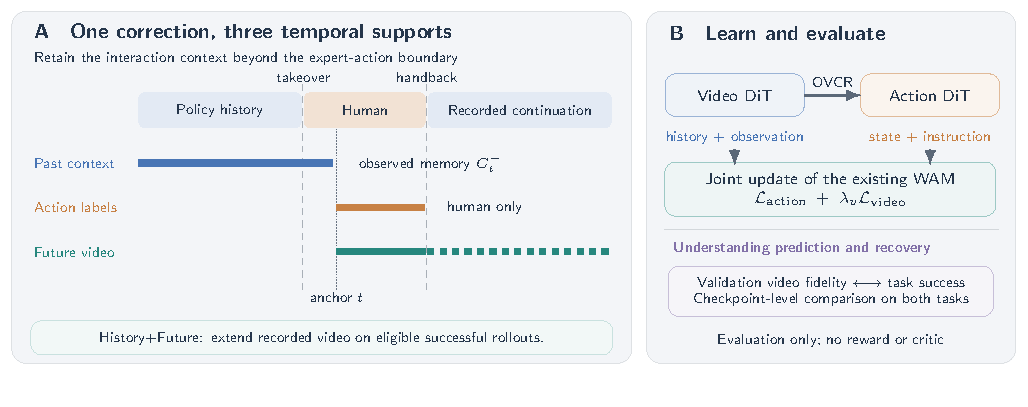
\includegraphics[width=\linewidth]{figures/method_overview.pdf}
\caption{Temporal support and supervision. History may precede takeover, expert actions remain within human control, and History+Future extends eligible recorded-video targets beyond handback. The existing backbone is jointly updated; predictive fidelity and task success are compared separately across checkpoints.}
\label{fig:method}
\end{figure*}

\subsection{Three Temporal Supports}
For each valid human-controlled training anchor $t\in[b,e]$, we construct history $C_t^-$, an action target with validity mask $m^a_{tj}$, and a future video target $C_t^+$ with eligibility indicator $m_t^v$. The action index $j$ enumerates the target chunk. A segment-only construction restricts all three to the human interval. Our protocol instead treats their boundaries separately:
\begin{equation}
\begin{aligned}
 C_t^-&=\operatorname{Past}(\tau,t;M,\Delta),\\
 m^a_{tj}&=\mathbf 1\{\text{target }j\text{ is valid in }[b,e]\},\\
 C_t^+&=\operatorname{Future}(\tau,t;K,\eta).
\end{aligned}
\label{eq:supports}
\end{equation}
Here $M$ is the history budget, $\Delta$ the sampling interval, $K$ the future horizon, and $\eta$ selects segment-only or extended targets. All supports remain within the same recorded interaction, and future targets never enter past conditioning.

\subsection{Preserving Context Before Takeover}
History $C_t^-$ may include observations before takeover $b$, preserving the approach to the corrected state. This prefix can include policy and earlier human control.

We compare segment-restricted and rollout-level history while holding the correction label fixed. History is a conditioning input, not an additional reconstruction objective. This preserves available context without assuming that more history always helps. For example, two similar images near an insertion opening can occur during the initial approach or after an unsuccessful descent. The preceding observations can help distinguish these situations and contextualize a human realignment. This is a motivation for retaining history, rather than an assumption that visual memory uniquely identifies the physical state.

\subsection{Observed Future Video Across Handback}
The basic variant supervises video only when a complete target fits within the correction segment; otherwise it retains action supervision and masks the direct video loss.

History+Future extends the video query beyond handback $e$ along the same successful mixed-control rollout, skipping system-hold frames. Incomplete targets remain masked. The extension never enlarges the expert-action mask in Eq.~\ref{eq:supports}.

Extended targets are recorded observations, potentially including autonomous execution and later interventions, rather than generated pseudo-labels. Prediction is self-supervised from images, while the overall procedure remains human-supervised and success-selected.

The video branch is not explicitly conditioned on arbitrary candidate actions; its predictions are visual continuations, not counterfactual control simulations.

Extending visual support exposes observations excluded by a short crop without adding expert actions or intervention anchors. The video ablation thus tests how the same corrective interactions are used, while changing both the amount and content of visual evidence.

\subsection{Behavioral Grounding of Predictive Learning}
The human intervention gives predictive post-training a behavioral anchor. The action objective specifies what the robot should imitate at a corrected state, while the video objective describes the observed continuation around that state. Keeping these signals distinct is important: a visually valid transition can follow an undesirable action, and a desirable corrective action can occur inside a trajectory that also contains failures. Assigning the entire interaction a single expert label would conflate these two cases.

Our construction instead couples selective action supervision with broader observation use. Successful-continuation selection narrows the visual targets to eligible mixed-control experience, while the human-only action mask preserves the source of expert behavior. This is an operational form of human-corrected predictive policy improvement: the learner revisits its deployment experience through behavioral correction and visual prediction. Here, self-improvement refers to post-training from the learner's interaction data with human guidance, rather than autonomous reward optimization or self-generated expert labels. The distinction is central to using a WAM's predictive capacity without treating its own executions as uniformly trustworthy.

\subsection{Joint Objective and Demonstration Replay}
We preserve the backbone's flow-matching objective~\cite{flow}. For a clean action or video latent $x$ and Gaussian noise $\epsilon$, the linear interpolation and velocity target are
\begin{equation}
 x_\sigma=(1-\sigma)x+\sigma\epsilon,\qquad
 u^*=\epsilon-x.
 \label{eq:flow}
\end{equation}
The corresponding networks predict the velocity under their visual, history, state, and language conditions. The action loss $\ell_i^a$ averages squared velocity error only over valid human action positions for correction samples; demonstration samples retain their ordinary valid actions. The video loss $\ell_i^v$ operates in the backbone's video latent space. Both retain the original noise-schedule weights, which we include in the per-sample losses.

For a training minibatch $B$, the masked objective is
\begin{equation}
 \widehat{\mathcal L}(B)=
 \frac{1}{|B|}\sum_{i\in B}\ell_i^a+
 \lambda_v\frac{\sum_{i\in B}m_i^v\ell_i^v}
 {\max(1,\sum_{i\in B}m_i^v)}.
 \label{eq:loss}
\end{equation}
Normalizing the video term over eligible samples avoids reducing its scale merely because a minibatch contains short action-only corrections. It also means that a nominal source ratio is not the same as the ratio of effective video supervision. All correction configurations here use $\lambda_v=1$; the video experiment changes target eligibility and extent, not whether a video objective exists.

Anchors are sampled from $q=\tfrac12\mathcal D+\tfrac12\mathcal H$. Demonstration replay retains nominal behavior alongside corrections, following the use of mixed experience in interactive learning~\cite{iwr,sirius}. Source proportions do not imply equal numbers of valid action or video targets.

Post-training updates the video DiT, action DiT, and routing parameters; text encoder and video autoencoder remain frozen. We add no actor, critic, or adapter.

\section{Experimental Design}
Our experiments ask whether corrective post-training improves task completion, how temporal support changes this improvement, and how held-out video fidelity relates to checkpoint-level task success. Table~\ref{tab:configs} defines the comparisons.

We organize the evidence around three complementary questions. First, does adding corrective interaction improve an otherwise demonstration-trained policy? The SFT--Segment-only comparison provides an intervention-learning reference. Second, does retaining temporal evidence beyond the takeover change performance? History and History+Future progressively expose the context and continuation available in the same recordings. Third, do predictive and behavioral improvements track one another? Held-out video evaluation examines this relationship without equating a realistic prediction with successful control. Together, these comparisons distinguish the value of correction data, the role of its temporal organization, and the interpretation of the resulting predictive representation.

\begin{table}[t]
\centering\small
\caption{Correction configurations, instantiated separately for both tasks. All have a video loss. ``Segment'' refers to its target boundary, not disabling the video branch. SFT is the original task SFT.}
\label{tab:configs}
\begin{tabular}{lll}
\toprule
Model & Correction history & Future video \\
\midrule
SFT & --- & --- \\
Segment-only & Within segment & Segment \\
History & Across takeover & Segment \\
History+Future & Across takeover & Extended \\
\bottomrule
\end{tabular}
\end{table}

\subsection{Robot, Tasks, and Data}
We use a low-cost SO101 arm with a fixed camera and a wrist camera. The policy receives images and robot state and predicts robot action chunks. The tasks are cylinder insertion and power-adapter manipulation with a final insertion stage.\footnote{To accommodate the SO101's force limits, we use a socket housing with its internal components removed, evaluating geometric alignment and insertion rather than electrical mating or the insertion-force requirements of an intact socket.} Full-task evaluation starts from the task's prescribed initial scene.

Each task SFT is trained for four epochs on its original demonstrations, without the later correction data. Human-gated interactions are then collected using the task policy. The human primarily intervenes after a deviation and teleoperates a correction. This makes recovery a natural evaluation target, without establishing that the learned policy cannot also avoid some errors. Training and evaluation use consistent camera setups within each task.

Training and validation corrections are separated by complete recorded rollouts rather than randomly splitting overlapping windows. This matters because different windows may reuse the same pre-takeover observations or post-handback future. Table~\ref{tab:data} reports the current training manifests. Counts describe valid human frames and segments, not the total amount of autonomous recording, and should not be interpreted as independent training examples of equal duration.

\begin{table}[t]
\centering\small
\caption{Correction training manifests. A rollout may contain multiple human segments.}
\label{tab:data}
\begin{tabularx}{\columnwidth}{@{}Xrr@{}}
\toprule
 & Cylinder & Power adapter \\
\midrule
Human-controlled frames & 3460 & 4289 \\
Human segments & 121 & 110 \\
Training rollouts & 82 & 67 \\
\bottomrule
\end{tabularx}
\end{table}

\subsection{Training and Controlled Comparisons}
Each correction variant starts from the same four-epoch task SFT. We use batch size 12 and learning rate $10^{-5}$ with cosine decay. Update budgets are 3285 steps for cylinder and 2664 for power adapter.

The history budget is six frames. Segment-only restricts correction history to the human segment rather than globally disabling memory. Cylinder Segment-only retains History's history stride and hold filtering; power-adapter Segment-only also changes these settings, so the latter Segment-only--History comparison tests a history-construction bundle.

History and History+Future share human action labels, history construction, source ratio, and update budget, and differ in visual continuation. Across deployment comparisons we hold camera setup, task instruction, normalization, action sampling settings, and chunk execution settings fixed.

\subsection{Full-Task Evaluation}
We evaluate unassisted task completion from shared task-specific initializations: 13 trials per model for cylinder and 20 for power adapter. Cylinder uses the first rollout at each initialization, excluding unequal extra repeats; this rule was clarified retrospectively. Partial insertions are failures. Table~\ref{tab:success} reports percentages.

\begin{table}[t]
\centering\small
\caption{Autonomous task success (\%). Segment-only uses segment-based correction context; History retains rollout history; History+Future additionally extends future-video supervision.}
\label{tab:success}
\begin{tabular}{lrr}
\toprule
Model & Cylinder & Power adapter \\
\midrule
SFT & 7.7 & 50.0 \\
Segment-only & 30.8 & \textbf{75.0} \\
History & 38.5 & 65.0 \\
History+Future & \textbf{46.2} & 55.0 \\
\bottomrule
\end{tabular}
\end{table}

\subsection{Held-Out Video Prediction}
We compare SFT, History, and History+Future on identical correction-start windows with recorded visual history: seven windows from four held-out cylinder rollouts and twelve from seven power-adapter rollouts. Video generation uses the same horizon, sampling budget, and seed across checkpoints. We report mean per-window RGB PSNR and MSE, excluding the clean conditioning frame; fixed- and wrist-camera scores use their respective image regions. Reference windows can extend beyond human control, and terminal reference frames are repeated when a window reaches the episode boundary.

Video fidelity is compared with independently measured task success at the checkpoint level. These are separate evaluation datasets, not paired video predictions and outcomes from the same robot trials.

\begin{figure*}[t]
\centering
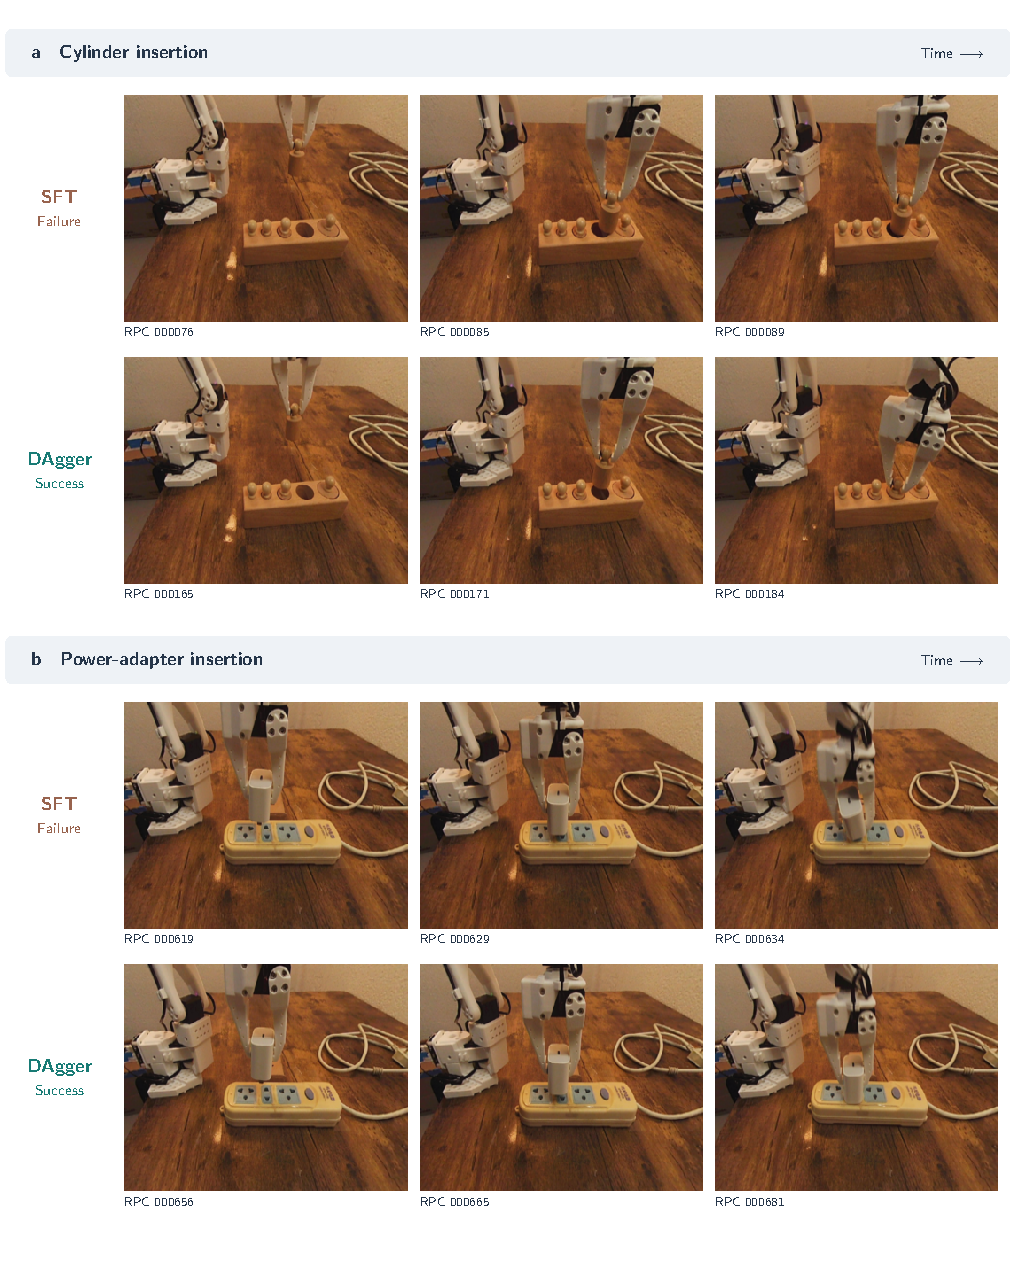
\includegraphics[width=.94\linewidth,height=.78\textheight,keepaspectratio]{figures/rollout_comparison.pdf}
\caption{Qualitative rollouts, progressing left to right. For each task, SFT is above DAgger. RPC identifiers preserve source-frame provenance; columns are not synchronized instants. These examples illustrate behavior rather than add success-rate measurements or a History--History+Future ablation.}
\label{fig:experiments}
\end{figure*}

\section{Results and Analysis}
\subsection{Task Completion and Corrective Behavior}
All corrective variants exceed SFT on both tasks (Table~\ref{tab:success}). Cylinder improves from 7.7\% to 30.8\%, 38.5\%, and 46.2\% for Segment-only, History, and History+Future; power adapter improves from 50.0\% to 75.0\%, 65.0\%, and 55.0\%.

Cylinder favors retained context and video extension, whereas power adapter favors Segment-only. The power-adapter Segment-only--History contrast includes the history-setting differences described above. History--History+Future more directly tests video support, but its direction is task dependent; it also changes both supervision coverage and target content.

Figure~\ref{fig:experiments} illustrates corrections after offset approaches and misaligned insertion attempts. The qualitative distinction is the response after deviation: the corrected policy can adjust its approach or move toward the opening rather than simply continue the unsuccessful motion. These observations complement full-task completion by illustrating the type of behavior supplied by intervention data. They do not by themselves separate error prevention from recovery or measure a continuous recovery region.

\subsection{Predictive Fidelity on Correction-Start Windows}
Corrective training improves video prediction on both tasks (Table~\ref{tab:video}). Relative to SFT, History and History+Future improve cylinder PSNR by 1.30 and 2.11 dB, exceeding SFT in all seven windows. On power adapter, the gains are 1.44 and 1.97 dB, with each variant exceeding SFT in eleven of twelve windows. History+Future has the highest mean fidelity for both tasks, although it does not win every window.

\begin{table}[t]
\centering\small
\caption{Held-out video fidelity. PSNR (dB) is higher-is-better; MSE uses 8-bit RGB and is lower-is-better. ``All'' scores the packed camera image; camera-specific scores use the indicated view.}
\label{tab:video}
\setlength{\tabcolsep}{3pt}
\begin{tabular}{lrrrr}
\toprule
Model & All & Fixed & Wrist & MSE \\
\midrule
\multicolumn{5}{l}{Cylinder} \\
SFT & 21.45 & 24.07 & 15.71 & 501.3 \\
History & 22.74 & 25.07 & 17.19 & 362.8 \\
History+Future & 23.56 & 26.02 & 18.09 & 303.9 \\
\midrule
\multicolumn{5}{l}{Power adapter} \\
SFT & 19.63 & 23.25 & 13.36 & 759.3 \\
History & 21.08 & 24.18 & 15.05 & 524.9 \\
History+Future & 21.61 & 24.87 & 15.52 & 469.4 \\
\bottomrule
\end{tabular}
\end{table}

Both camera views improve. On power adapter, History+Future gains 2.16 dB at the wrist and 1.62 dB at the fixed camera relative to SFT. This establishes a view-dependent difference, but without stage-specific labels it does not localize the gain to contact or alignment. Importantly, the predictive improvement is evaluated on held-out interactions rather than the training corrections. Agreement across camera views and most validation windows suggests that the mean gains are not confined to a single favorable view or example. It does not establish that pixel fidelity captures the small geometric differences that decide an insertion outcome.

\subsection{How Video Prediction May Support Error Recovery}
Two observations suggest coupled predictive and behavioral adaptation. First, History improves held-out correction-video fidelity despite limited direct video supervision from short corrections. Since the current video-context pathway remains jointly trainable, behavioral supervision may also adapt predictive representations. Second, History+Future further improves video fidelity on both tasks. This is consistent with learning more informative visual continuations, but the behavioral consequences differ.

For cylinder, SFT, History, and History+Future have the same ordering in video fidelity and task success. For power adapter, History achieves 65.0\% completion and History+Future 55.0\%, despite History+Future's higher PSNR (21.61 versus 21.08 dB). Thus, better reference-video prediction is not a sufficient indicator of better control. These are descriptive comparisons across three checkpoints per task, not a causal or statistically general relationship.

Joint forecasting can make visual representations useful for action prediction~\cite{videovla}. Our results motivate this mechanism for recovery, while revealing a prediction--execution gap: a more accurate continuation of held-out interaction need not improve autonomous contact behavior. We do not search generated videos to choose actions; the analysis concerns predictive learning within the existing WAM. Isolating its causal contribution requires targeted loss or feature-pathway ablations.

This distinction matters for interpreting a WAM's imagined future. Reference-video evaluation measures agreement with a particular recorded continuation, whereas autonomous success depends on the states induced by the updated policy and its subsequent responses. A representation can improve the former without supplying the corrective precision needed for the latter. The two tasks therefore provide complementary evidence: cylinder is consistent with useful predictive--behavioral coupling, while power adapter shows why predictive fidelity should be evaluated alongside execution rather than used as its substitute.

\section{Discussion and Limitations}

\textbf{Interactive post-training as selective learning.} Beyond the Takeover treats deployment as a source of complementary supervision rather than a homogeneous set of expert trajectories. Human corrections identify behavior worth imitating, while recorded visual context supports predictive learning around those corrections. This offers a way to use the WAM's joint modeling structure without assuming that autonomous execution is consistently correct. The general design principle is to separate control ownership from the temporal extent of usable observations; its effectiveness beyond this backbone remains an open empirical question.

\textbf{Visibility.} The adapter can obscure its mating interface, whereas the cylinder offers a more visible alignment gap. Insertion studies motivate complementary tactile sensing under visual uncertainty~\cite{visiontouch}; temporal prediction can also help track occluded objects~\cite{temporalplanning}. Visibility is therefore a plausible boundary condition, but we have neither controlled occlusion nor measured hallucinations, and cannot attribute the task difference to either.

\textbf{Scope of the diagnostic.} Prediction--performance relationships have been studied in visual model-based learning and joint video--action models~\cite{modelspixels,videovla}. Unlike action-conditioned policy evaluation~\cite{worldgym}, our analysis compares reference-video fidelity with separate deployments. Three checkpoint rankings cannot establish causality or make PSNR a general success surrogate.

Our evaluation uses limited initializations, one training seed per configuration, and one video sampling seed. Shared source rollouts, repeated reference tails, human intervention choices, and successful-continuation filtering limit independence and generality. Additional tasks and targeted action/video-loss ablations are needed to test the proposed mechanisms.

\section{Conclusion}
We present Beyond the Takeover, an interactive post-training framework that adapts a memory-based WAM through human corrections embedded in their observed temporal context. Separating history, expert action labels, and future-video targets allows short interventions to support predictive policy adaptation. Corrective training improves observed completion on both insertion tasks, while temporal-support ablations reveal task-dependent benefits. Video prediction improves on both tasks, but the adapter reveals that higher predictive fidelity need not yield higher task success. These findings motivate studying both the contribution and the limits of predictive representations for recovery.

%---------- acknowledgements ----------
\section*{ACKNOWLEDGEMENTS}
This work was supported by the National Key R\&D Program of China (Grant No. 2026YFE0104400), the National Natural Science Foundation of China (NSFC, Grant No. 52401393 and No. 12502288), the Natural Science Foundation of Hangzhou, Zhejiang Province, China (Grant No. 2025SZRJJ1217), and the Guangdong Philosophy and Social Science Foundation (Grant No. GD26YJY18). We also gratefully acknowledge the LoongForge team from Baidu AI Cloud for computational resource support.
% Review the scope of this factual disclosure against the final retained material.
\bibliographystyle{IEEEtran}
\bibliography{references}
\end{document}
